\documentclass[a4paper,french]{paper}
\usepackage{../../_latex_assets/villemejane_iogs_ceti}

%Informations about this document 
%------------------------------------------
\def\module{Ingénierie Electronique pour le Traitement de l'Information}
\def\moduleAbrege{6N-047-SCI / IéTI}
\def\annee{}

\def\titre{TD 3 / Modéliser et corriger des systèmes}
\author{Julien VILLEMEJANE}

\subtitle{TD 3}
\institution{LEnsE / Institut d'Optique Graduate School}

\title{\titre}
\begin{document} 
%Beginning First Page. 
%------------------------------------------
\enteteThematiqueObligatoire{}

%Beginning Content. 
%------------------------------------------
\vspace{-1cm}
%%%%%%%%%%%%%%%%%%%
\encadreTDExo{1 - Rebouclage d'un ALI}{
\subsection*{Modèle de l'ALI en boucle ouverte}
On peut modéliser un amplificateur linéaire intégré par un système du premier ordre de type :

$$A(p) = \frac{V_S(p)}{\varepsilon(p)} = \frac{A_0}{1 + \frac{p}{\omega_c}}$$

où $V_S(p)$ est la tension de sortie de l'ALI et $\varepsilon(p) = V^+(p) - V^-(p)$ la tension différentielle d'entrée.

\begin{enumerate}
	\item Quelle relation existe-t-il entre $A_0$, $\omega_c$ et $GBP$ (le produit gain bande-passante de l'ALI) ?
	\item Tracez la réponse en fréquence asymptotique en gain de ce système.
	\item Calculez le gain statique et la pulsation (ou fréquence) caractéristique de ce système si on suppose que $A_0 = 10^5$ et $GBP = 3\operatorname{MHz}$ ?
\end{enumerate}

%%%%%%%%%%%%%%%%%%%%%%%%%%%%%%%%%%%%%
\subsection*{Rebouclage en suiveur}

\begin{enumerate}
	\item Proposez un schéma bloc pour un \textbf{montage suiveur}.
	\item Calculez la fonction de transfert en boucle fermée de ce montage. 		
	\item Que valent à présent le gain statique et la pulsation caractéristique de ce système (pour les mêmes valeurs de $A_0$ et $GBP$) ?
	\item Tracez la réponse en fréquence de ce nouveau système.
\end{enumerate}
}


\textbf{\large ALI en boucle ouverte} 

\textbf{Produit gain et bande-passante} 

Le produit gain bande-passante est constant, ainsi : $A_0 \cdot f_c = GBP$, on a alors que : $w_c = 2 \cdot \pi \cdot GBP / A_0$


\textbf{Réponse en fréquence}

Ce système peut se modéliser sous forme de schéma bloc de la façon suivante :

\begin{center}
	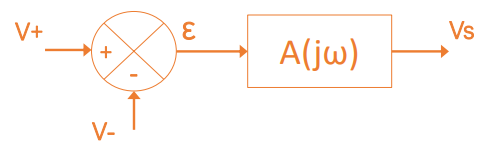
\includegraphics[width=7cm]{images/TD/correction_ALI_BO.png}
\end{center}	
		
On obtient le comportement d'un passe-bas du premier ordre dont la fréquence de coupure vaut $\omega_c$. 
		
\begin{center}
	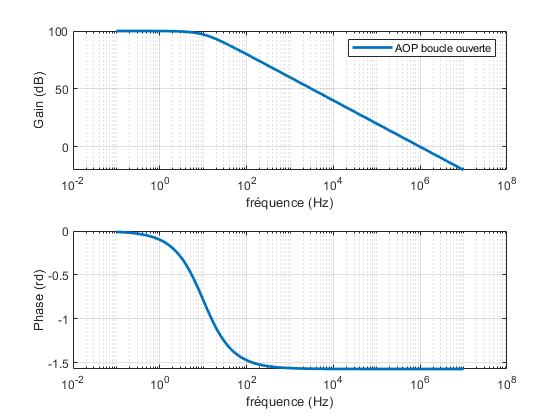
\includegraphics[width=12cm]{images/TD/correction_ALI_BO_Bode.png}
\end{center}	
 
\textbf{Gain statique et pulsation de coupure}

Le gain statique (dans la bande-passante) vaut $G_0 = 20 \cdot \log{A_0} = 100\operatorname{dB}$.
		
La bande-passante vaut : $f_c = GBP / A_0 = 30\operatorname{Hz}$.


\qquad


\textbf{\large ALI rebouclé en suiveur} 

\textbf{Schéma bloc} 

\begin{center}
	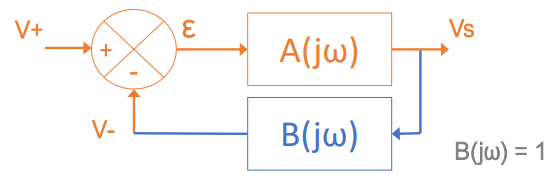
\includegraphics[width=8cm]{images/TD/correction_ALI_BFunit.png}
\end{center}

\textbf{Fonction de transfert} 

On a $H(p) = A(p) / (1 + A(p) \cdot B(p))$ avec $A(p)$ la fonction de transfert de l'ALI et $B(p) = 1$.
		
On obtient alors : 
		
$$H(p) = \frac{\frac{A_0}{1 + \frac{p}{\omega_c}}}{1 + \frac{A_0}{1 + \frac{p}{\omega_c}}}$$
		
Après simplification, on obtient : 
		
$$H(p) = \frac{A_0}{1 + A_0} \cdot \frac{1}{1 + \frac{p}{\omega_c \cdot (1 + A_0)}}$$


\textbf{Gain statique et pulsation de coupure}

Le gain statique vaut : $H_0 = \frac{A_0}{1 + A_0} \approx 1$.
		
La pulsation caractéristique vaut : $\omega_0 = \omega_c \cdot (1 + A_0)$. 
		
donc $f_0 = f_c \cdot (1 + A_0) = GBP \cdot \frac{1 + A_0}{A_0} \approx 3\operatorname{MHz}$.


\textbf{Réponse en fréquence}

On obtient le comportement d'un passe-bas du premier ordre dont la fréquence de coupure vaut $\omega_c \cdot (1 + A_0)$. 

\begin{center}
	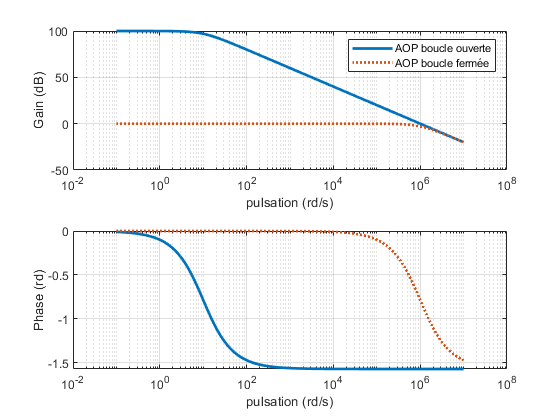
\includegraphics[width=12cm]{images/TD/correction_ALI_BFunit_Bode.png}
\end{center}

\newpage
%------------------------------------------
%%%%%%%%%%%%%%%%%%%
\encadreTDExo{2 - Modèle de l'oscilloscope}{
L'oscilloscope et son système de mesure peut donc être modélisé par un dipôle $RC$ comme représenté ci-dessous.

\begin{center}
	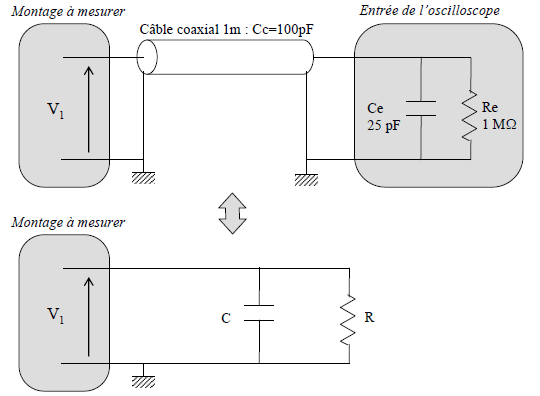
\includegraphics{images/TD/TD5_ex2.png}
\end{center} 
}

%------------------------------------------
%%%%%%%%%%%%%%%%%%%
\encadreTDExo{2a - Modèle de l'oscilloscope}{

L'entrée de mesure d'un oscilloscope est généralement modélisée par un dipôle constitué d'une résistance $R_e$ de $1\operatorname{M\Omega}$ en parallèle avec un condensateur ayant une capacité $C_e$ de $25\operatorname{pF}$ (cette valeur peut varier légèrement d'un type d'oscilloscope à un autre).

Par ailleurs, le câble coaxial utilisé pour relier le point de mesure à l'oscilloscope présente une capacité parasite $C_c$ de $100\operatorname{pF}$ (pour 1 m de câble). On négligera la résistance du câble devant $R_e$.

Déterminez les valeurs de $R$ et de $C$ du modèle équivalent.
}

$R = R_e$ et $C = C_e + C_c$ (capacités en parallèle)

Ainsi : 

$$Z = \frac{\frac{R}{j C \omega}}{R + \frac{1}{j C \omega}} = \frac{R}{1 + j R C \omega}$$


%------------------------------------------
%%%%%%%%%%%%%%%%%%%
\encadreTDExo{2b - Sonde compensée pour oscilloscope}{

L'impédance du dipôle de mesure peut donner une \textbf{mesure erronée} de la tension $V_1$. C'est pourquoi il convient d'utiliser une sonde correctement réglée afin d'augmenter l'impédance du dipôle de mesure. Cette sonde est constituée d'un câble coaxial analogue au précédent et d'une tête de sonde comprenant une résistance $R_s$ de $9\operatorname{M\Omega}$ en parallèle avec un condensateur $C_s$ variable entre $5$ et $50\operatorname{pF}$. Le schéma complet du montage est alors le suivant.


\begin{center}
	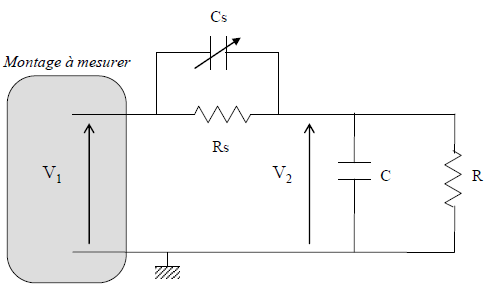
\includegraphics{images/TD/TD5_ex2b.png}
\end{center}

\begin{enumerate}
	\item Faites une étude asymptotique du montage lorsque $\omega$ tend vers 0 et vers l'infini. En déduire le comportement du montage pour ces deux cas extrêmes.
	\item Calculez la fonction de transfert $T(j\omega{}) = V_2/V_1$ de ce montage.
	\item Tracez le diagramme asymptotique de Bode en amplitude et en phase de $T(j\omega{})$ pour $C_s = 5\operatorname{pF}$.
	\item Tracez le diagramme asymptotique de Bode en amplitude et en phase de $T(j\omega{})$ pour $C_s = 50\operatorname{pF}$.
	\item Quelle valeur faut-il donner à $C_s$ pour que la tension $V_2$ soit proportionnelle à la tension $V_1$ quelque soit la fréquence du signal alternatif sinusoïdal à mesurer ?
	\item Exprimez l'impédance d'entrée de l'ensemble "sonde + oscilloscope" vue des bornes de la tension $V_1$.
\end{enumerate}
}


\textbf{\large Comportement asymptotique} 

\textbf{Lorsque $\omega \rightarrow 0$}
	
alors $1/C \omega >> R$, on obtient un pont diviseur avec $R$ et $R_S$ et 
	
$$V_2 = V_1 \cdot \frac{R}{R + R_S}$$
	
\medskip

\textbf{Lorsque $\omega \rightarrow \infty$}
	
alors $1/C \omega << R$, on obtient un pont diviseur avec $C$ et $C_S$ et 
	
$$V_2 = V_1 \cdot \frac{\frac{1}{j C \omega}}{\frac{1}{j C \omega} + \frac{1}{j C_S \omega}}$$
	
$$V_2 = V_1 \cdot \frac{C_S}{C + C_S}$$

\qquad

\textbf{\large Fonction de transfert}

On peut utiliser le principe du pont diviseur (en notation complexe) :

$$T = \frac{V_2}{V_1} = \frac{Z}{Z + Z_S}$$

avec $Z = R / (1 + j R C \omega)$  et $Z_S = R_S / (1 + j R_S C_S \omega)$

On obtient ainsi :

$$T =  \frac{\frac{R}{1 + j R C \omega}}{\frac{R}{1 + j R C \omega} + \frac{R_S}{1 + j R_S C_S \omega}} $$

$$T = \frac{R}{1 + j R C \omega} \cdot \frac{(1 + j R C \omega) \cdot (1 + j R_S C_S \omega)}{R + R_S + j R R_S (C + C_S) \omega} $$


$$T = \frac{R}{R + R_S} \cdot \frac{1 + j R_S C_S \omega}{1 + j \frac{R R_S}{R + R_S} (C + C_S) \omega} $$

\medskip

On obtient ainsi 2 fréquences distinctes :

\begin{center}
\begin{Large}
\begin{tabular}{cc}
$f_1 = \frac{1}{2 \pi R_S C_S}$ &
$f_2 = \frac{R + R_S}{2 \pi R R_S (C + C_S)}$\\
\end{tabular}
\end{Large}
\end{center}


\qquad

\textbf{\large Diagramme asymptotique - cas $C_S = 5\operatorname{pF}$}


AN : $f_1 = 3.5\operatorname{kHz}$ et $f_2 = 1.3\operatorname{kHz}$

\begin{center}
	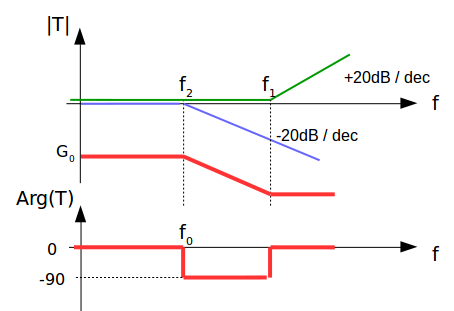
\includegraphics{images/TD/TD5_ex2_c1.png}
\end{center}

\begin{center}
	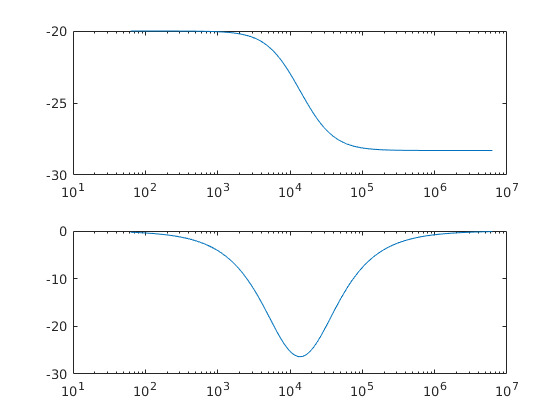
\includegraphics{images/TD/TD5_ex2_cs5pf.png}
\end{center}

\qquad

\textbf{\large Diagramme asymptotique - cas $C_S = 50\operatorname{pF}$}

AN : $f_1 = 350\operatorname{Hz}$ et $f_2 = 1\operatorname{kHz}$

\begin{center}
	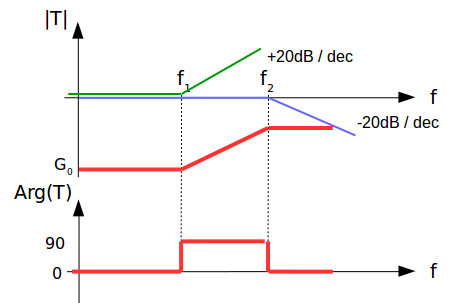
\includegraphics{images/TD/TD5_ex2_c2.png}
\end{center}

\begin{center}
	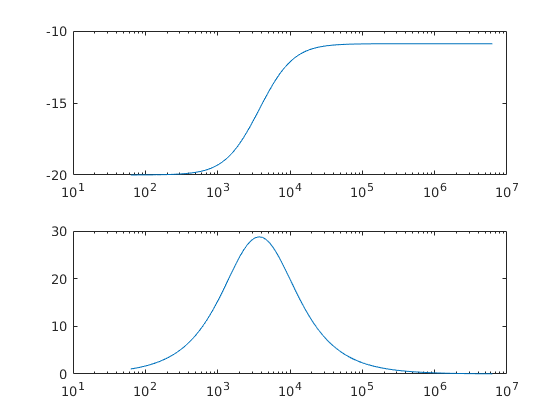
\includegraphics{images/TD/TD5_ex2_cs50pf.png}
\end{center}

\qquad

\textbf{\large Cas idéal}

Il faut que $f_1 = f_2$

$$R_S C_S = \frac{R_S R (C_S + C)}{R_S + R}$$

$$C_S = C \cdot \frac{R}{R_S}$$

AN : $C_S = 13.8 \operatorname{pF}$

\begin{center}
	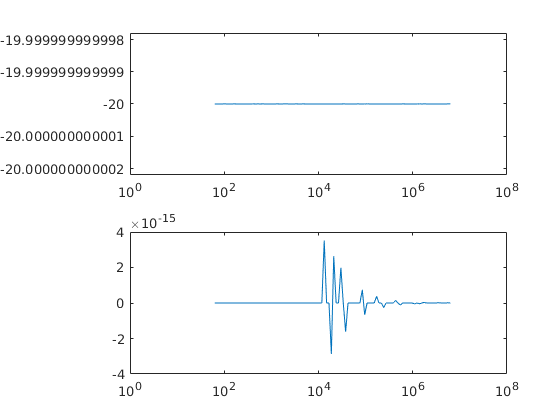
\includegraphics{images/TD/TD5_ex2_cscomp.png}
\end{center}

\qquad

\textbf{\large Impédance d'entrée}

$Z_{eq} = Z + Z_S$ avec $Z = R / (1 + j R C \omega)$  et $Z_S = R_S / (1 + j R_S C_S \omega)$


\begin{center}
	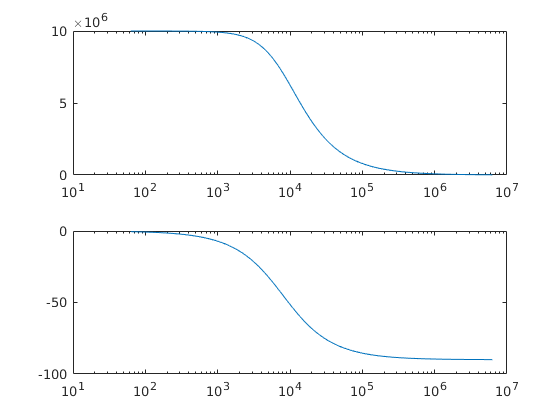
\includegraphics{images/TD/TD5_ex2_z.png}
\end{center}


\end {document}